\documentclass[tikz,border=3pt]{standalone}
\usepackage[utf8]{inputenc}
\usepackage[T1]{fontenc}
\usepackage{libertinus}
\usepackage{amsmath,amssymb}
\usepackage{pgfplots}
\pgfplotsset{compat=1.18}
\usetikzlibrary{arrows.meta}
\definecolor{UGblue}{RGB}{0,51,102}
\begin{document}
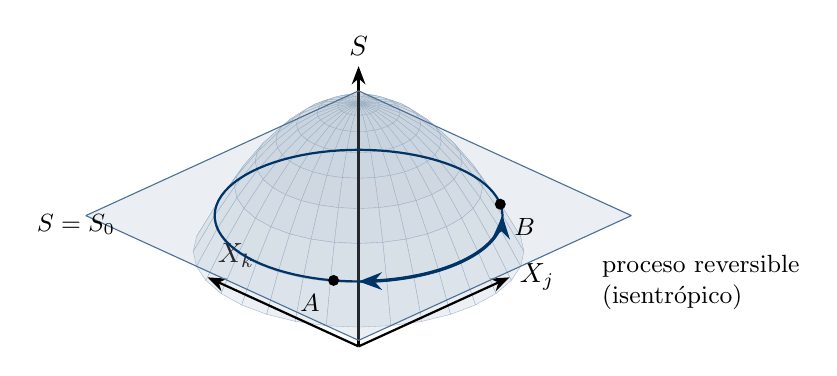
\begin{tikzpicture}
\begin{axis}[hide axis,view={-45}{34},width=9.5cm,height=9cm,xmin=-1.6,xmax=1.6,ymin=-1.6,ymax=1.6,zmin=0,zmax=1.6,z buffer=sort,clip=false,>=Stealth,
  colormap={s}{color(0cm)=(UGblue!6) color(1cm)=(UGblue!18)}]
\addplot3[surf,shader=flat,draw=UGblue!40,line width=0.12pt,domain=0:1.2,y domain=0:360,samples=9,samples y=33,z buffer=sort]
  ({x*cos(y)},{x*sin(y)},{1.3-0.55*x*x});
\draw[->,thick] (axis cs:0,0,0) -- (axis cs:1.55,0,0) node[right] {$X_j$};
\draw[->,thick] (axis cs:0,0,0) -- (axis cs:0,1.55,0) node[above right] {$X_k$};
\draw[->,thick] (axis cs:0,0,0) -- (axis cs:0,0,1.5) node[above] {$S$};
\addplot3[patch,patch type=rectangle,shader=flat,fill=UGblue!35,fill opacity=0.22,draw=UGblue!70,line width=0.4pt] coordinates {(-1.4,-1.4,0.7) (1.4,-1.4,0.7) (1.4,1.4,0.7) (-1.4,1.4,0.7)};
\draw[thick,UGblue] plot[domain=0:360,samples=90,variable=\t] (axis cs:{1.0445*cos(\t)},{1.0445*sin(\t)},{0.7});
\draw[<->,very thick,UGblue] plot[domain=225:315,samples=30,variable=\t] (axis cs:{1.0445*cos(\t)},{1.0445*sin(\t)},{0.7});
\node[circle,fill,inner sep=1.4pt,label={[font=\small]below left:$A$}] at (axis cs:-0.8556,-0.5991,0.7000) {};
\node[circle,fill,inner sep=1.4pt,label={[font=\small]below right:$B$}] at (axis cs:0.8556,-0.5991,0.7000) {};
\node[font=\small] at (axis cs:-1.55,1.35,0.7) {$S=S_0$};
\node[font=\small,align=left,anchor=west] at (axis cs:1.5,-0.9,0.2) {proceso reversible\\(isentrópico)};
\end{axis}
\end{tikzpicture}
\end{document}
